\section{Интервалы основанные на стандартном нормальном распределении}
Пусть $\widehat{\theta}$ есть оценка параметра $\theta$ методом подстановки, $\widehat{\text{se}}$ оценка его стандартной ошибки. Рассмотрим стандартный нормальный доверительный интервал $[ \widehat{\theta} - z^{(1 - \alpha)} \cdot \widehat{\text{se}}, \widehat{\theta} - z^{(\alpha)}\cdot \widehat{\text{se}}]$. Граничные точки этого интервала можно описать способом, который особенно удобен для бутстреп вычислений. Пусть $\widehat{\theta}^{*}$  есть случайная величина, взятая из распределения $\mathrm{N}(\widehat{\theta}, \widehat{\text{se}}^{*})$:
\begin{gather}\label{13.1}
\widehat{\theta}^{*}\sim \mathrm{N}(\widehat{\theta}, \text{se}^{2}).
\end{gather}
Тогда $\widehat{\theta}_{\text{lo}} = \widehat{\theta}  - z^{(1 - \alpha)} \cdot \widehat{\text{se}} $ и $\widehat{\theta}_{\text{up}} = \widehat{\theta}  - z^{(\alpha)} \cdot \widehat{\text{se}}$  являются $100\cdot \alpha$ и $100 \cdot (1 - \alpha)$ процентилями $\widehat{\theta}^{*}$. Другми словами:

\begin{gather}\label{13.2}
\widehat{\theta}_{\text{lo}} = \widehat{\theta}^{*(\alpha)} = 100 \cdot \alpha \ \text{процентиль распределения} \  \widehat{\theta}^{*}, \\
\widehat{\theta}_{\text{up}} = \widehat{\theta}^{*(1 - \alpha)} = 100 \cdot (1 - \alpha) \  \text{процентиль распределения} \  \widehat{\theta}^{*}.
\end{gather}

Например, посмотрим на данные с мышами из таблицы 2.1, пусть $\widehat{\theta} = 86.85$, для 7 мышей. Бутстреп стандартная ошибка для $\widehat{\theta}$ равна 25.23, так что если мы выберем $\alpha = 0.05$, тогда нормальный стандартный $90\%$ доверительный интервал для истинного среднего  $\theta$  составляет $[86.85 - 1,645 \cdot 25.23, \ 86.85 + 1.645 \cdot 25.23] = [45.3,\ 128.4]$.

\begin{figure}[H]
\center{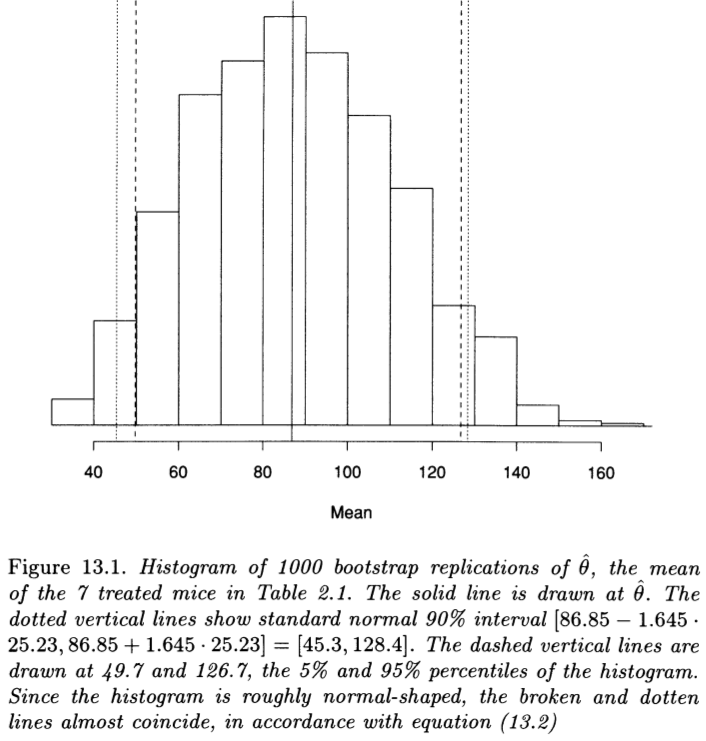
\includegraphics[width=1 \linewidth]{13/f13.1.png}}
\end{figure}

На рисунке 13.1 показана гистограмма 1000 бутстреп репликаций $\widehat{\theta}^{*}$. Похоже на нормальное распределение, поэтому согласно уравнению (\ref{13.2}), $5\%$ и $95\%$ процентили этой гистограммы должны быть примерно в точках 45.3 и 128.4 соответственно. Это неплохое приближение, как показано в таблице 13.1, $5\%$ и $95\%$ процентили равны 49.7 и 126.7.
\begin{figure}[H]
\center{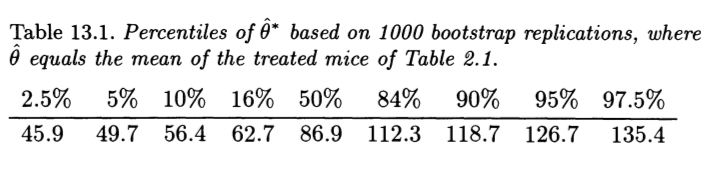
\includegraphics[width=1 \linewidth]{13/f13.2.png}}
\end{figure}